\documentclass[11pt]{scrartcl}
\usepackage[utf8]{inputenc}
\usepackage[spanish]{babel}
\usepackage[parfill]{parskip}
\usepackage{graphicx}
\usepackage{float}
\usepackage{listings}

\lstdefinestyle{Shell}{delim=[il][\bfseries]{BB}}

\title{\textbf{R}}
\subtitle{Language and environment for stadistical computing graphics}
\author{Ricardo Garc\'a Fern\'andez}
\date{\today}

\begin{document}

\maketitle

\section{Introducci\'on}

\textbf{R} es un lenguaje y un entorno para datos y gr\'aficos estad\'isticos.
Se basa en el Lenguaje \textbf{S}. 
Ross Ihaka y Robert Gentleman.
Licencia  GNU v2.

\section{Propiedades}

Se est\'a constituyendo como est\'andar 'de facto'.
Bibliotecas gestionadas a trav\'es de un repositorio para facilitar la integraci\'on.

\section{Instalaci\'on}

\begin{lstlisting}[style=Shell]
	bash> apt-get install r-base r-cran-rmysql
\end{lstlisting}

\subsection{GUI}

Se ha desarrollado una herramienta gr\'afica para poder hacer la entrada en el ecosistema R m\'as sencilla, debido a que el primer contacto parece un poco tosco. R-commander\footnote{http://www.rcommander.com/} es un ejemplo.

R-commander install:

\begin{lstlisting}[style=Shell]
	bash> R
	R> install.packages('Rcmdr', dep = T)
	R> library(Rcmdr)
\end{lstlisting}

\section{Commandos}

Aqu\'i vemos una peque\~na muestra de los comando b\'asicos asociados a R. Necesarios en la toma de contacto de cualquier lenguaje de programaci\'on.

Ayuda:

\begin{lstlisting}[style=Shell]
	R> help(functionname)
	R> help.search(''word'')
	R> apropos(''word'')
\end{lstlisting}

Inside my library:

\begin{lstlisting}[style=Shell]
	R> library(help=MASS)
\end{lstlisting}

\section{Scripts}

En el lenguaje \emph{R} tambi\'en podemos ver algunos ejemplos a través de un script.

\begin{lstlisting}
library(RMySQL)

con = dbConnect(MySQL(), user='root', pass='admin', \
dbname='fm3_audacity_cvsanaly2_cvs_scm')

results = dbGetQuery(con, "select committer_id, count(*)\
 as ncommits from scmlog group by committer_id order by ncommits desc")

jpeg("barplot_audacity.jpg")

barplot(log10(results[,2]), names.arg = \
as.character(results[,1]), col = "blue")

dev.off()
\end{lstlisting}

\section{Gr\'aficas}

La ejecuci\'on del script anterior convierte los resultados obtenidos de la consulta en un gr\'afico. Representa los commits (cambios en el c\'odigo fuente del progama) de cada committer (usuario que hace el commit) del repositorio (gestor de las versiones del c\'odigo fuente) de Audacity\footnote{http://audacity.sourceforge.net/} ordenados de forma descendiente. El resultado se puede ver en la figura~\ref{fig:commits}.

\begin{figure}[H]
    \begin{center}
    \centering
    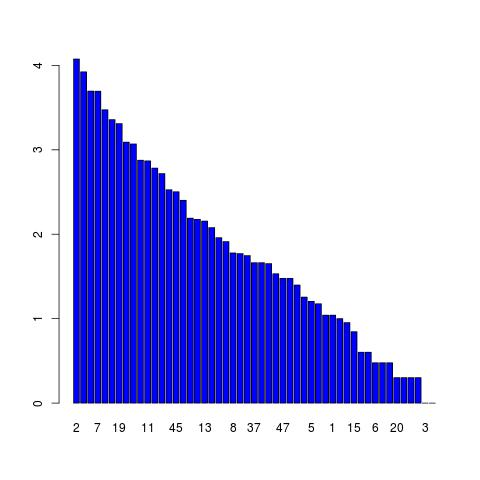
\includegraphics[scale=0.7]{scripts/barplot_audacity.jpg}
    \caption{}
    \label{fig:commits}
    \end{center}
\end{figure}

\begin{thebibliography}{9}

\bibitem{rinformation}
  The Comprehensive R Archive Network,\\
  http://www.cran.r-project.org/

\end{thebibliography}
\end{document}